\chapter{Background}

% TODO: "Por favor, evite utilizar o texto em 1a pessoa, do singular ou plural. Não irei corrigir esse tipo uso daqui pra frente. Significa que é necessário modificar o texto para se adaptar a 3a pessoa."


Neste capítulo será apresentado os trabalhos existentes sobre análise de dados e detecção de outliers com algoritmos e estratégias de como usar essa abordagem para melhorar a análise dos dados e aumentar a quantidade e a qualidade das informações que podemos obter dos datasets.

\section{GeoGuide}

Visando melhorar a análise de dados espaciais e a abordagem por orientação para esse tipo de dado, o GeoGuide \cite{omidvarTehrani2017} é um framework interativo que visa destacar para o analista um subconjunto de $k$ pontos espaciais interessantes, baseado nos feedbacks \textit{implícito} (ex.: rastreamento do mouse) e \textit{explícito} (ex.: pontos clicados) do analista, que podem não terem sido vistos dado o montante de informação aparente na sua tela. Esse framework leva em consideração duas importantes métricas para poder destacar um subconjunto. A primeira é a \textbf{relevância} de cada ponto para o ponto selecionado pelo analista considerando os atributos não espaciais desses pontos. O segundo é a \textbf{diversidade} geográfica para que assim possa expandir a área de análise do usuário em busca de possíveis novas regiões de seu interesse.

Todo esse processo pode ser utilizado em datasets espaciais genéricos, contanto que cada ponto do conjunto tenha duas características: atributos geográficos (ex.: latitude e longitude) e atributos \textit{metadados} de domínio do dataset. Por exemplo, a plataforma Airbnb\footnote{\it http://www.airbnb.com} tem datasets abertos sobre as casas disponíveis para alugar e cada uma delas tem atributos geográficos e \textit{preço, nome do hospedador e disponibilidade} como seus atributos metadados que são específicos para cada tipo de dataset como podemos ver na Figura \ref{fig:geoguide-example-airbnb}. Utilizando essa abordagem, o GeoGuide é o primeiro framework interativo eficiente para destaque de dados espaciais, combinando o feedback do analista com as métricas de relevância e diversidade para mostrar a ele um subconjunto de pontos interessantes que podem ter sido deixado de lado durante sua análise.

Essa ferramenta construída foi fruto de um projeto de pesquisa realizado no Instituto Federal de Educação, Ciência e Tecnologia do Rio Grande do Norte (IFRN) em parceria com a Universidade de Grenoble realizado por alunos do curso superior de Tecnologia em Análise e Desenvolvimento de Sistemas (TADS), dentre os quais me incluo, e serviu de base para a construção deste trabalho visando melhorias na abordagem já existente.

% TODO: "Paragrafo importante para contextualizar seu trabalho."

\begin{figure*}[t]
	\centering
	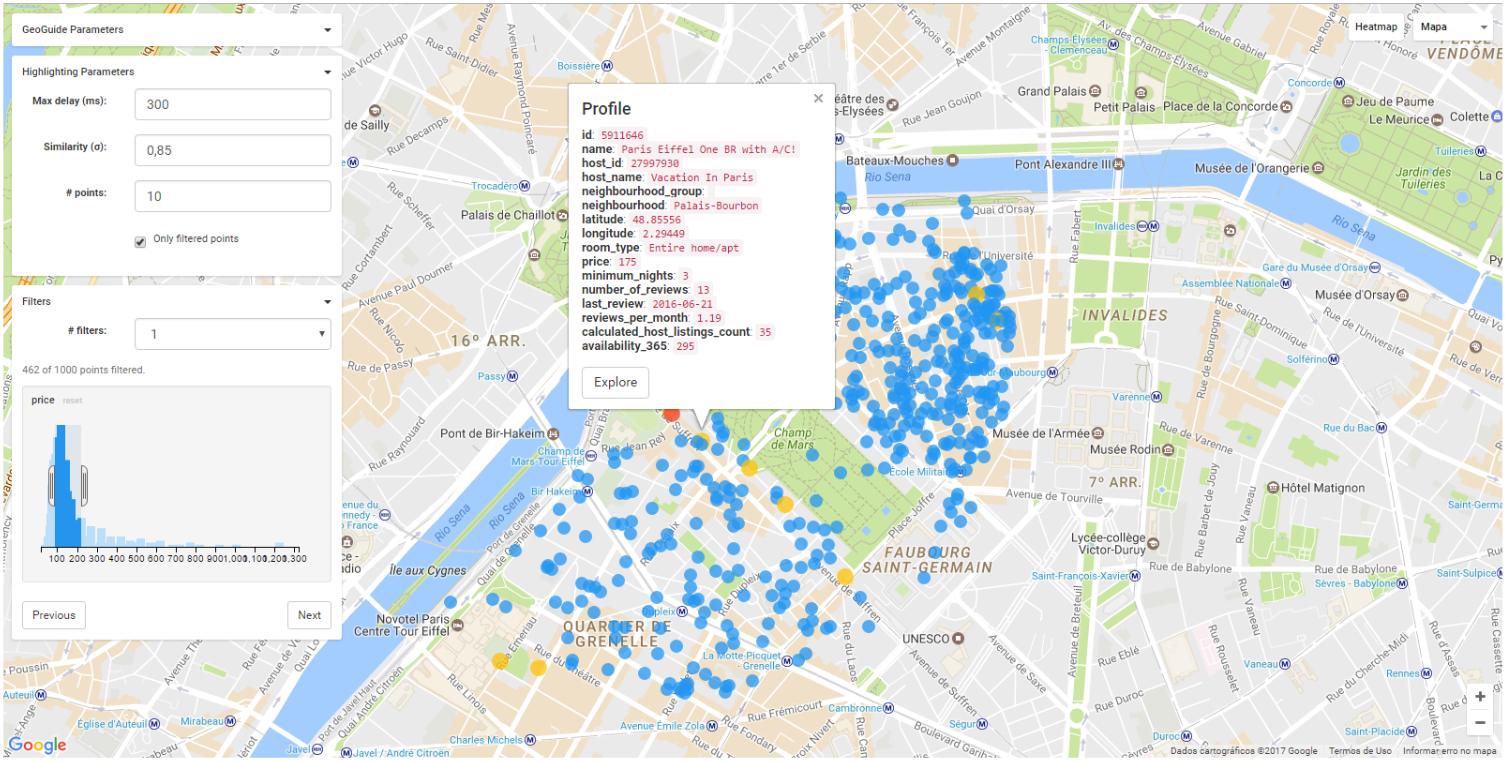
\includegraphics[width=\textwidth]{images/geoguide-example-airbnb}
	\caption{Figura do GeoGuide no dataset do Airbnb - Cidade de Paris}
	\label{fig:geoguide-example-airbnb}
	\vspace{-10pt}
\end{figure*}

\section{Outliers}

No campo da estatística, Outliers são quando se encontram ``discrepâncias'' num determinado conjunto de dados, ou seja, quando alguém acha um valor atípico ou muito fora da distribuição normal daquele conjunto. Por exemplo, quando um pesquisador quer monitorar a temperatura de sua CPU durante um certo intervalo de tempo e foi percebido que a variação de temperatura foi entre 34 ºC e 45 ºC com máxima de 48 ºC e mínima de 27 ºC e no meio dessa amostragem são encontrados registros pontuais de 0 ºC, isso é caracterizado como um outlier e, muito provavelmente, será interpretado como um defeito do equipamento que realizou a coleta da temperatura da CPU.

Entretanto, existem diversas formas de interpretar um Outlier além de um erro da coleta, como: um dado que pertença à uma população diferente da amostra, um dado defeituoso, um dado que esteja numa área em que certa teoria não é válida ou até, quando a amostra é muito grande, é normal haver pequenas quantidades de outliers naquele grupo. Em casos em que são provados que não é culpa de um equipamento defeituoso de coleta ou que não foi uma falha humana, é extremamente importante entender o porquê daquele outlier, pois não é interessante para o pesquisador simplesmente removê-lo ou ressignificá-lo definindo-lhe um novo valor, já que essa mudança pode comprometer a validade da pesquisa e, caso aconteça, é de extrema importância que tudo isso seja documentado para registro dessas alterações.

Assim como as tecnologias da informação melhoram e aumentam continuamente seu poder computacional, uma grande variedade de algoritmos para detecção de outliers tem surgido e vem sendo aplicado em diferentes contextos com diversas características, sendo que a escolha para um desses algoritmos é baseada no domínio do problema. A seguir será apresentado alguns desses algoritmos com uma breve explicação sobre cada um.

\subsection{Z-Score}

Z-Score \cite{doi:10.1111/j.1540-6261.1968.tb00843.x} é um dos métodos mais simples para detecção de outliers em um dataset. É um método paramétrico que leva em consideração somente um atributo por execução e é necessário a entrada de um valor limite (geralmente um valor entre 2,5 e 3,5) para poder definir se um determinado dado pode ser considerado como um outlier ou não. Esse método é adequado para pequenos datasets que seguem a distribuição Gaussiana.

\subsection{DBSCAN}

É um algoritmo de clusterização de dados espaciais baseado em densidade \cite{Ester:1996:DAD:3001460.3001507} que pode ser aplicado em datasets os quais não se pode presumir qual a sua distribuição e que aceita datasets multidimensionais (com 3 ou mais dimensões). Entretanto, é necessário a entrada de um parâmetro (MinPts) que definirá quantos pontos são minimamente necessários para se formar um \textit{cluster}. Portanto, se o tamanho do conjunto mudar, esse parâmetro terá que ser atualizado, caso contrário, o DBSCAN pode se tornar ineficiente.

\subsection{Isolation Forests}

É um algoritmo de detecção de outliers \cite{IsolationForests} que usa um dos conceitos de aprendizagem de máquina que são as chamadas árvores de decisão. Ele leva em consideração a distribuição de probabilidade do dataset, seu foco é na busca de outliers, ao invés de categorizar os atributos considerados normais, e são necessários poucos parâmetros de entrada (isso facilita a configuração e uso do algoritmo). Porém, é mais conveniente utilizá-lo em datasets de médio porte.

\subsection{FDC}

É uma abordagem de algoritmo baseado em profundidade \cite{Johnson:1998:FCD:3000292.3000332} para detecção de outliers em datasets 2D que se baseia no conceito do algoritmo ISODEPTH \cite{RUTS1996}. O FDC computa os primeiros $k$ contornos de profundidade (os pontos que podem ser considerados outliers) restrigindo a uma pequena parte do dataset completo. Dessa forma, é mais eficiente por não ter que calcular no dataset completo e, portanto, mais fácil de escalar para grandes datasets de duas dimensões.

\subsection{HOD}

É um método de detecção de outlier baseado em distância \cite{Xu2016} que surge para superar os métodos baseados em estatísticas, já que na vasta maioria dos datasets a distribuição de probabilidade não é conhecida. Dessa forma, o método busca por outliers baseado na sua distância em relação aos seus vizinhos e se essa distância é maior que um parâmetro de entrada predefinido, então esse ponto é considerado um outlier. Entretanto, se já existe um cluster de outliers no dataset, isso pode afetar a detecção em algoritmos baseado em distância, para isso que serve o conceito HOD (\textit{Hidden Outlier Detection}) do algoritmo que visa encontrar outliers mesmo quando eles estão agrupados em quantidades suficientes para formação de um cluster.

\subsection{ORCA}

É um algoritmo baseado em distância \cite{Bay:2003:MDO:956750.956758} que otimiza um algoritmo simples de loop aninhado (que são algoritmos de complexidade exponencial os quais são extremamente ineficientes quando utilizados em grandes datasets) pela remoção de possíveis \textit{non-outliers} durante sua execução \cite{Knorr:1999:FIK:645925.671529,Knorr:2000:DOA:764212.764218,Ramaswamy:2000:EAM:335191.335437}. Dessa forma, ao invés de processar o dataset por completo, ele vai removendo cálculos que serão desnecessários, já que o ponto não vai ser considerado um outlier. A partir dele, novas pesquisas têm surgido para refinar mais esse conceito. 

\subsection{Linearization}

É um algoritmo baseado em distância \cite{10.1007/3-540-45681-3_2} que detecta outliers calculando a soma das distâncias de um ponto em relação aos seus vizinhos, chamando isso de \textit{peso}, e definindo os outliers como os pontos com os maiores pesos no dataset. Dessa forma, é um algoritmo eficiente de complexidade linear tanto em relação ao número de pontos como ao número de dimensões. Para ajudar a calcular esses outliers mais eficientemente, o algoritmo utiliza o conceito da \textit{curva de Hilbert}.

\subsection{RBRP}

É um algoritmo de alta perfomance para datasets multidimensionais que é baseado nas distâncias entre os pontos para poder definir quais são os outliers no dataset \cite{Ghoting2006}. Sua diferença para os outros algoritmos baseado em distância é que ele se torna mais eficiente quando executado em dataset com múltiplas dimensões, sua escalabilidade é aproximadamente linear para o número de dimensões e logarítmica para o número de pontos no dataset.

\subsection{LOF}

É um algoritmo baseado em densidade que adiciona um novo conceito na busca por outliers: o \textit{Local Outlier Factor (LOF)} \cite{Breunig:2000:LID:335191.335388}, que é um grau de propensidade que aquele ponto tem de ser um outlier e dessa forma o processo de definição de outlier não é mais binário, mas sim algo gradual. Com isto, a abordagem não é mais sobre um ponto ser outlier ou não, mas sim o ``quão outlier'' esse ponto é em relação ao dataset. O \textit{outlier factor} é local no sentido que somente os vizinhos daquele ponto são levados em consideração para definir seu fator.

\subsection{ABOD}

É um algoritmo de detecção de outlier baseado em ângulo \cite{Kriegel:2008:AOD:1401890.1401946} que é focado em datasets de altas dimensões, diferente de outros algoritmos baseado em distância que acabam prejudicados quando o dataset tem muitas dimensões. Sua abordagem é baseado no cálculo do grau do ângulo entre os diferentes vetores de um ponto com os seus vizinhos. Com isto, pontos mais centralizados dentro do cluster terão esse grau calculado com um valor maior, já os pontos mais próximos da borda terão esse valor um pouco menor e o possíveis outliers terão esse grau com valores muito pequenos, já que eles geralmente estarão distantes do cluster em uma direção particular. 

\vspace{25pt}

Baseado nos algoritmos apresentados, nós organizamos cada um de acordo com a resposta para nossas questões propostas sobre algoritmos de detecção de outliers no geral. As questões são: \textbf{I} \textit{É paramétrico?}; \textbf{II} \textit{Qual é a abordagem?}; \textbf{III} \textit{É escalável em termos de performance?}; \textbf{IV} \textit{É escalável em termos de múltiplas dimensões?} e \textbf{V} \textit{Ele recebe algum argumento?}. O resultado é apresentado na Tabela \ref{table:algorithms-comparison}.

\begin{table}[!h]
	\centering
	\begin{tabular}{|l|l|l|l|l|l|}
		\hline
		\textbf{Algorithms}               & \textbf{I} & \textbf{II}             & \textbf{III} & \textbf{IV} & \textbf{V} \\ \hline
		\textbf{Z-Score}                  & Sim        & Baseado em Modelo       & Não          & Não         & Sim        \\ \hline
		\textbf{DBSCAN}                   & Não        & Baseado em Densidade    & Não          & Sim         & Sim        \\ \hline
		\textbf{Isolation Forests}        & Sim        & Baseado em Profundidade & Não          & Sim         & Não        \\ \hline
		\textbf{FDC}                      & Não        & Baseado em Profundidade & Sim          & Não         & Não        \\ \hline
		\textbf{Hidden Outlier Detection} & Não        & Baseado em Distância    & Sim          & Sim         & Sim        \\ \hline
		\textbf{ORCA}                     & Não        & Baseado em Distância    & Não          & Sim         & Sim        \\ \hline
		\textbf{Linearization}            & Não        & Baseado em Distância    & Sim          & Sim         & Sim        \\ \hline
		\textbf{RBRP}                     & Não        & Baseado em Distância    & Sim          & Sim         & Sim        \\ \hline
		\textbf{LOF}                      & Não        & Baseado em Densidade    & Não          & Sim         & Sim        \\ \hline
		\textbf{ABOD}                     & Não        & Altas Dimensões         & Não          & Sim         & Não        \\ \hline
	\end{tabular}
	\caption{Comparação dos Algoritmos de Detecção de Outlier apresentados}
	\label{table:algorithms-comparison}
\end{table}

Cada questão tem uma motivação específica para estar na Tabela \ref{table:algorithms-comparison}. A questão \textbf{I} é sobre a distribuição de probabilidade do dataset. Se o algoritmo é paramétrico, então nós podemos assumir a distribuição de probabilidade do dataset baseado em um conjunto fixo de parâmetros. A questão \textbf{II} serve para classificar cada algoritmo baseado na abordagem que ele utiliza para indicar se um dado é um outlier ou não, as opções são: \textit{Baseado em Modelo}, \textit{Baseado em Densidade}, \textit{Baseado em Profundidade}, \textit{Baseado em Distância} e \textit{Altas Dimensões}. A questão \textbf{III} é relativa a performance computacional de cada algoritmo, se o tempo de execução do algoritmo não é comprometido de acordo com o crescimento do dataset, significa que ele é escalável em termos de performance. A questão \textbf{IV} é sobre a performance de cada algoritmo também, mas nesse caso é relacionado ao crescimento de dimensões do dataset. Por fim, a questão \textbf{V} indica se o algoritmo requer algum argumento de entrada para processar o dataset, isso é importante pois se o algoritmo requer muitos argumentos pode se tornar um problema de precisão quando o dataset aumentar.

\section{Análise dos algoritmos}

Após a categorização e o agrupamento dos algoritmos analisados baseado nas questões propostas, nós analisamos cada algoritmo e como ele se encaixaria com nossa proposta de trabalho.

O algoritmo Z-Score é de uma complexidade muito simples comparado ao outros analisados, porém sua abordagem serve somente para os datasets em que podemos inferir qual seria sua distribuição de probabilidade e nossa proposta é trabalhar com datasets genéricos e pouco conhecido. Junto dele também temos o algoritmo FDC que não funciona para múltiplas dimensões (3D ou mais), mas a nossa proposta pretende atingir datasets sem limites de atributos.

O DBSCAN tem uma abordagem interessante, mas precisa ser calibrado de acordo com a mudança do dataset e isso é muito sensitivo, podendo influenciar muito os resultados com pequenas alterações nos parâmetros de entrada. Além disso seus atributos precisam ser escalados antes da sua execução.

O algoritmo Isolation Forests é recomendado somente em datasets que conhecemos sua distribuição, dessa forma, assim como o Z-Score, não é recomendado para a nossa proposta com datasets genéricos.

O método Hidden Outlier Detection é mais elaborado e complexo, sendo o mais indicado em casos em que existem muitos outliers a ponto de formar uma espécie de cluster com eles, porém, é como se ele fosse ``um passo a mais'' no processo de detecção e não podemos indicar que os datasets terão essa estrutura.

O ORCA é um algoritmo que foca em melhorar a performance dos algoritmos que utilizam loops aninhados para encontrar outliers, o Linearization é um algoritmo que utiliza o conceito da \textit{curva de Hilbert} para ajudar no seu processo e o RBRP é um algoritmo que tem eficiência muito boa em datasets de múltiplas dimensões, mas esses 3 algoritmos são de abordagens baseadas em \textit{Distância}, de forma que isso possa não ser o mais indicado nas regiões de pequenas áreas que queremos utilizar no nosso trabalho.

O algoritmo LOF é de uma abordagem de \textit{Densidade} que propõe um conceito de ``não-binariedade'' na definição de um outlier com a atribuição de um grau para cada ponto indicando o ``quão outlier'' ele pode ser naquele conjunto. Isso nos chama atenção para poder trabalhar com nuances de outliers.

Por fim, o algoritmo ABOD é focado em datasets com múltiplas dimensões e com uma abordagem única no nosso grupo analisado que é justamente ser muito específico para datasets com essas características. Entendemos que ele é um pouco mais complexo para a nossa proposta e que não podemos predizer se essa característica prevalecerá no uso da nossa ferramenta.